%!TEX root = ../../../main.tex
\chapter{Technische Alternativen}\label{chap:lokal}
\noindent\textit{Verfasser: Daniel Schmal}
\medskip

Das vorherige Kapitel endete mit drei Anforderungen. Nötig sind eine lokale
Rückfallebene für die wichtigsten Funktionen, offene Schnittstellen, die einen
Wechsel ermöglichen, und ein geregelter Ausstieg, wenn der Support endet
(vgl. Abschnitt~\ref{sec:cloud-zwischenfazit}). Dieses Kapitel prüft, wie weit
quelloffene Software diese Anforderungen schon heute erfüllt. Statt alle
Lösungen aufzuzählen, folgt es dem Beispiel eines Haushalts, dessen
Saugroboter wie im Fall Neato nur über App und Herstellerkonto voll
funktioniert (vgl. Abschnitt~\ref{sec:cloud-neato}). Der Saugroboter eignet
sich dafür, weil er sensible Daten aus der Wohnung mit Funktionen verbindet,
die an der Cloud hängen. Die Überlegungen lassen sich auf andere
Haushaltsgeräte übertragen. Industrielle Anlagen bleiben außen vor, da die
Arbeit die individuelle Ebene digitaler Souveränität betrachtet. Die These
lautet, dass sich die Kontrolle technisch zurückgewinnen lässt. Je tiefer der
Eingriff in ein Gerät aber geht, desto mehr Verantwortung und Risiko tragen die
Nutzer selbst.

\section{Lokale Steuerung}\label{sec:lokal-steuerung}

\subsection{Open Source als Gegenentwurf}\label{sec:lokal-opensource}

Die Informatikerin Irene Weber, Professorin an der Hochschule für Angewandte
Wissenschaften Kempten, versteht Open-Source-Software als Software, die ihre
Funktionsweise offenlegt und unabhängig von ihrem Produzenten verwendet werden
kann \cite[S.~1]{weber:2026}. Für Anwender folgt daraus, dass kein Hersteller
unbemerkt Funktionen einbauen kann, die etwa Daten abgreifen, und dass er
weder die Nutzungsbedingungen ändern noch den Umstieg auf eine Cloud-Version
erzwingen kann. Auch einen Vendor-Lock-in können Anwender vermeiden, weil sie
die Software notfalls selbst weiterführen können, was in der Praxis allerdings
aufwendig ist \cite[S.~47\,f.]{weber:2026}. Genau diese Eigenschaften fehlten
in den Fällen aus Kapitel~\ref{chap:cloud}.

Das Projekt Home Assistant hat diese Grundsätze in seiner Vision des
\enquote{Open Home} für das Smart Home konkretisiert. Geräte sollen lokal
funktionieren, ihre Daten über lokale Schnittstellen bereitstellen und
dauerhaft nutzbar bleiben
\cite[Abschn.~\enquote{Privacy}, \enquote{Choice}, \enquote{Sustainability}]{homeassistant:2021}.
Diese drei Werte entsprechen der Daten-, Entscheidungs- und
Anwendungssouveränität. Getragen wird das Projekt heute von der Open Home
Foundation, nach deren Grundsätzen Cloud-Dienste optional bleiben müssen
\cite[Abschn.~\enquote{Privacy}]{ohf:oj}. Anders als bei den Abo-Modellen aus
Abschnitt~\ref{sec:cloud-haas} ist die Cloud hier ein Zusatz und keine
Voraussetzung. Souveränität bedeutet also nicht, auf die Cloud zu verzichten,
sondern selbst über sie zu entscheiden.

\subsection{Lokale Zentralen}\label{sec:lokal-zentralen}

Eine lokale Zentrale dreht die Architektur aus
Abschnitt~\ref{sec:cloud-endpunkt} um. Die Steuerlogik und alle Automationen
laufen auf einem Rechner im eigenen Heimnetz, etwa einem Raspberry Pi. Home
Assistant spricht die Geräte lokal an und weicht nur auf die Cloud aus, wenn
es keine andere Möglichkeit gibt
\cite[Abschn.~\enquote{All your smart home data stays local}]{homeassistant:oj}.
Die Alternative openHAB verfolgt dasselbe Ziel
\cite[Abschn.~\enquote{No Cloud Required\dots}]{openhab:oj}.
Tabelle~\ref{tab:lokal-architektur} stellt beide Architekturen gegenüber.

\begin{table}[htbp]
  \centering
  \caption{Cloud-zentrierte und lokale Smart-Home-Architektur im Vergleich}
  \label{tab:lokal-architektur}
  \footnotesize
  \setlength{\tabcolsep}{4pt}
  \renewcommand{\arraystretch}{1.25}
  \begin{tabularx}{\textwidth}{@{}>{\raggedright\arraybackslash}p{3.2cm}
      >{\raggedright\arraybackslash}X
      >{\raggedright\arraybackslash}X@{}}
    \toprule
    \textbf{Merkmal} & \textbf{Cloud-zentriert (Hersteller-App)}
      & \textbf{Lokal (eigene Zentrale)} \\
    \midrule
    Ort der Steuerlogik & Server des Herstellers
      & Rechner im eigenen Heimnetz \\
    Speicherort der Daten & Beim Hersteller, z.\,B. Wohnungskarten
      & Im Haushalt, Weitergabe nur bei bewusster Freigabe \\
    Internetausfall & Grundfunktionen fallen teilweise oder ganz aus
      & Automationen laufen weiter, nur der Fernzugriff fällt aus \\
    Ende des Herstellers & Gerät verliert Funktionen oder wird wertlos
      & Lokal angebundene Geräte bleiben nutzbar \\
    Updates und Wartung & Durch den Hersteller, auch gegen den Willen
      der Nutzer & Durch die Nutzer selbst \\
    Einrichtungsaufwand & Gering, App installieren und Konto anlegen
      & Hoch, eigene Hardware, Konfiguration und Pflege \\
    \bottomrule
  \end{tabularx}
  \par\smallskip
  \raggedright\scriptsize
  Quelle: Eigene Darstellung auf Basis von
  \cite{homeassistant:2021,homeassistant:oj,openhab:oj} sowie
  Kapitel~\ref{chap:cloud}.
\end{table}

Für den Beispielhaushalt ändert eine Zentrale allein jedoch wenig. Hat der
Saugroboter keine lokale Schnittstelle, kann auch Home Assistant ihn nur über
die Hersteller-Cloud ansprechen. Fällt die Cloud weg, fällt der Roboter auch
in der Zentrale aus, und wie schnell ein solcher Zugang gesperrt werden kann,
zeigt der Fall Chamberlain (vgl. Abschnitt~\ref{sec:cloud-lockin}). Eine
Zentrale macht also nur nutzbar, was die Geräte an Offenheit mitbringen.

\subsection{Offene Standards}\label{sec:lokal-standards}

Diese Offenheit können offene Funkstandards liefern. Geräte mit Zigbee oder
Z-Wave bilden ein Mesh-Netz, brauchen keine eigene Internetverbindung und
arbeiten mit Zentralen verschiedener Hersteller zusammen
\cite[Abschn.~\enquote{Consumers}]{csa:zigbee},
\cite[Abschn.~\enquote{Z-Wave Technology Essentials}]{zwave:oj}.

Für den Lock-in ist vor allem der neuere Standard Matter wichtig. Die
Connectivity Standards Alliance (\acrshort{CSA}) entwickelt ihn als offenen
und lizenzfreien Standard. Ein Matter-Netz arbeitet im Heimnetz auch ohne
Verbindung zum Internet vollständig eigenständig \cite[S.~1, 7]{belli:2024}. Über
die Funktion \enquote{Multi-Admin} legen Nutzer selbst fest, welche Plattformen
auf ein Gerät zugreifen dürfen, auch mehrere gleichzeitig
\cite[Abschn.~\enquote{Security and Privacy}]{csa:matterfaq}.
Seit Version~1.2 aus dem Jahr 2023 gehören auch Saugroboter dazu
\cite[Abschn.~\enquote{Nine New Device Types}]{csa:2023}. Wer heute einen
Matter-fähigen Roboter kauft, kann ihn also lokal und unabhängig von der
Hersteller-App steuern.

Dem Beispielhaushalt hilft das nur, wenn der Hersteller Matter nachträglich
per Update einführt. Zudem behalten viele Hersteller erweiterte Funktionen
ihrer eigenen App vor. Belli, Barsocchi und Palumbo sehen außerdem keine
Gewähr, dass Matter nicht zu einem Standard wird, den wenige große Anbieter
kontrollieren. Schon der Zugang zur jeweils entstehenden Fassung der
Spezifikation setzt eine Mitgliedschaft für 20\,000 US-Dollar im Jahr voraus
\cite[S.~24]{belli:2024}. Das sind genau die Gatekeeper, vor denen die
\acrshort{UBA}-Studie warnt (vgl. Abschnitt~\ref{sec:cloud-lockin}). Matter erleichtert damit vor allem
den Wechsel zwischen großen Ökosystemen, garantiert aber keinen Weiterbetrieb
nach dem Supportende. Für bereits gekaufte, geschlossene Geräte bleibt nur der
Eingriff in das Gerät selbst.

\section{Freie Software für geschlossene Geräte}\label{sec:lokal-firmware}

\subsection{Das Beispiel Saugroboter}\label{sec:lokal-valetudo}

Für Saugroboter bietet Valetudo einen solchen Eingriff. Das Projekt versteht
sich als Cloud-Ersatz für einen rein lokalen Betrieb und ausdrücklich nicht als
eigene Firmware \cite[Abschn.~\enquote{What is Valetudo?}]{valetudo:2025}. Die
Hersteller-Software bleibt auf dem Roboter und steuert weiter Motoren und
Sensoren. Valetudo läuft daneben und bildet die Cloud des Herstellers nach
\cite[Abschn.~\enquote{Robots that aren't supported}]{valetudo:robots}.
Abbildung~\ref{fig:lokal-valetudo} stellt beide Betriebsarten gegenüber.

\begin{figure}[htbp]
  \centering
  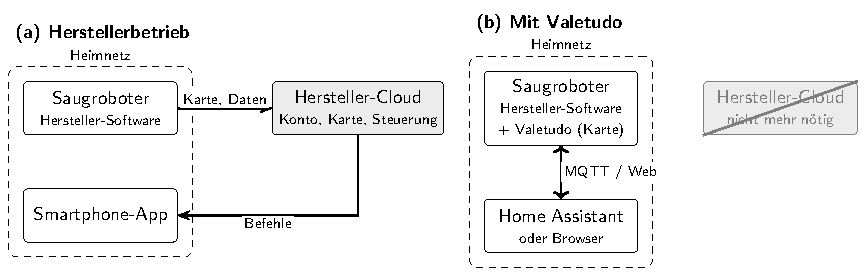
\includegraphics[width=\textwidth]{images/chapter3/valetudo-datenfluss.pdf}
  \caption{Datenfluss eines Saugroboters im Herstellerbetrieb und mit Valetudo}
  \label{fig:lokal-valetudo}
  \par\smallskip
  \raggedright\scriptsize
  Quelle: Eigene Darstellung auf Basis von \cite{valetudo:2025,valetudo:robots}.
\end{figure}

Der Weg beginnt für den Beispielhaushalt mit einer Prüfung, denn Valetudo
läuft nur auf einer festen Liste von rund 50 Modellen, vor allem von Dreame,
Roborock und Xiaomi \cite{valetudo:robots}. Neato-Roboter gehören nicht dazu.
Steht das Modell auf der Liste, muss der Roboter \enquote{gerootet} werden,
also über eine Sicherheitslücke vollen Zugriff auf sein Betriebssystem
erhalten. Dafür sind Kenntnisse in Linux, Kommandozeile und Netzwerktechnik
nötig \cite[Abschn.~\enquote{Skills}]{valetudo:rooting}.

Danach ändert sich der Alltag mit dem Gerät grundlegend. Die Wohnungskarte
liegt auf dem Roboter statt beim Hersteller, und bedient wird er über eine
Weboberfläche im Heimnetz. Raumreinigung und Sperrzonen bleiben erhalten. Über
das Protokoll Message Queuing Telemetry Transport (\acrshort{MQTT}) lässt sich
der Roboter zudem in Home Assistant einbinden, sodass er etwa startet, sobald
alle Bewohner das Haus verlassen haben
\cite[Abschn.~\enquote{What is Valetudo?}, \enquote{What can Valetudo do?}]{valetudo:2025}.
Kamerabilder verlassen die Wohnung nicht mehr, der Roboter reinigt auch nach
einer Abschaltung der Herstellerserver weiter, und Updates, die Funktionen
nachträglich hinter eine Bezahlschranke verschieben, sind ausgeschlossen
\cite[Abschn.~\enquote{Your data stays at home}, \enquote{No server dependency}, \enquote{No forced updates}]{valetudo:why}.
Damit erfüllt der Haushalt alle drei Anforderungen aus
Abschnitt~\ref{sec:cloud-zwischenfazit}, die er beim Kauf nicht hatte.

Dafür gibt er aber auch etwas auf. Die Hersteller-App funktioniert ohne Cloud
nicht mehr, und für Sicherheitsupdates ist der Haushalt nun selbst
verantwortlich \cite[Abschn.~\enquote{Downsides}]{valetudo:why}. Zudem hängt er
jetzt von einem anderen Akteur ab. Valetudo wird im Wesentlichen von einer
einzigen Person als Hobby entwickelt, die das Projekt nicht vergrößern will
\cite[Abschn.~\enquote{Valetudo is a garden}]{valetudo:oj}. Das eng verwandte
Projekt Nimbus nennt diesen Entwickler als früheren Mitwirkenden
\cite[Abschn.~\enquote{Free your vacuum from the cloud}]{nimbus:oj}. Offener
Code kann also weitergeführt werden, wenn ein Projekt endet. Ob das geschieht,
hängt aber von wenigen Freiwilligen ab. Weber sieht darin ein allgemeines Problem, denn
vielen Open-Source-Projekten fehlt eine dauerhafte Finanzierung, um ihre
Software sicher und aktuell zu halten \cite[S.~53]{weber:2026}.

\subsection{KI-Assistenten als neues Werkzeug}\label{sec:lokal-ki}

Für die meisten anderen Geräte gibt es kein Projekt wie Valetudo. Nur bei
einfachen Steckdosen und Sensoren lässt sich die Firmware oft durch freie
Alternativen wie Tasmota oder ESPHome ersetzen \cite{tasmota:oj,esphome:oj}.
Wer ein anderes Gerät befreien wollte, musste es bislang selbst analysieren,
und das war Fachleuten vorbehalten.

In jüngster Zeit verschiebt sich diese Grenze. Nutzer setzen
Programmierassistenten auf Basis künstlicher Intelligenz (\acrshort{KI}) wie
Claude Code ein, um Geräte zu analysieren und neue Software dafür zu schreiben.
Ein Entwickler ließ so die App und die Bluetooth-Kommunikation seines
Heimspeichers untersuchen und band ihn danach lokal an Home Assistant an
\cite{singh:2026}. Andere entfernten Werbung und vorinstallierte Apps von
Smart-TVs oder nahmen Geräte wieder in Betrieb, die ihre Hersteller aufgegeben
hatten. Einem Nutzer genügte dafür die Modellnummer seines Fernsehers
\cite{koebler:2026}. Dass der Ansatz trägt, zeigt auch eine Studie von
Humphries. Mit einem \acrshort{KI}-Assistenten rekonstruierte er das
verschlüsselte, nicht dokumentierte Verwaltungsprotokoll der von Apple
aufgegebenen AirPort-Router und schätzt den Aufwand auf vier bis fünf Tage
statt mehrerer Monate \cite[S.~1]{humphries:2026}. Die Befreiung von Geräten, bisher ein Werkzeug weniger
Fachleute, wird damit für deutlich mehr Menschen erreichbar. Der
Beispielhaushalt könnte so auch einen Roboter wieder nutzbar machen, für den
es kein fertiges Projekt gibt.

Eine ehrliche Einschätzung muss aber die Risiken benennen. Erstens bleibt viel
menschliches Urteil nötig. Selbst in Humphries' Studie hinterließ der Assistent
Geräte in ungültigen Zuständen, die von Hand zurückgesetzt werden mussten, und
einzelne Versuche ließen Router schwach gesicherte WLAN-Netze ausstrahlen
\cite[S.~3]{humphries:2026}. Zudem lässt sich so nur nachbauen, was lokal
vorhanden ist. Daten, die allein in der Hersteller-Cloud lagen, lassen sich
nicht zurückholen \cite[S.~4]{humphries:2026}, im Fall Neato etwa die
Wohnungskarten (vgl. Abschnitt~\ref{sec:cloud-neato}). Zweitens ist die erzeugte Software oft unsicher. In
einer Studie der Universität Stanford schrieben Teilnehmende mit
\acrshort{KI}-Assistent deutlich unsichereren Code als ohne und hielten ihn
trotzdem häufiger für sicher \cite[S.~2785]{perry:2023}. Drittens entsteht ein
Widerspruch, denn die Assistenten sind meist Cloud-Dienste großer Anbieter.
Wer sie nutzt, gibt Gerätedaten an einen weiteren Dienst weiter und tauscht so
die Abhängigkeit vom Hersteller teilweise gegen eine Abhängigkeit vom
\acrshort{KI}-Anbieter. Lokal betriebene, quelloffene Modelle vermeiden das,
verlangen aber leistungsfähige eigene Hardware und Fachwissen. Das Bundesamt
für Sicherheit in der Informationstechnik (\acrshort{BSI}) und die französische
Cybersicherheitsbehörde (\acrshort{ANSSI}) betonen deshalb, dass
\acrshort{KI}-Assistenten erfahrene Entwickler nicht ersetzen und erzeugter
Code immer geprüft werden muss \cite[S.~3, 12]{bsi:2024ki}. Genau diese
Prüfung können Laien aber nicht leisten.

\subsection{Was bleibt für die Nutzer}\label{sec:lokal-kritik}

Für den Beispielhaushalt fällt die Bilanz gemischt aus. Er gewinnt die
Kontrolle über Daten und Funktionen zurück, riskiert aber die Garantie
\cite[Abschn.~\enquote{Installing Valetudo}]{valetudo:start} und im
schlimmsten Fall einen Totalschaden, wenn beim Rooten etwas schiefgeht
\cite[Abschn.~\enquote{Skills}]{valetudo:rooting}. \acrshort{KI}-Assistenten
scheinen das nötige Fachwissen zu ersetzen, doch gerade wo es fehlt, bleiben
ihre Fehler unsichtbar. Und für die Sicherheit ist der Haushalt nun selbst
verantwortlich. Damit verschärft sich das Problem aus
Abschnitt~\ref{sec:cloud-zwischenfazit}, dass Weiterbetrieb nicht dasselbe ist
wie Sicherheit. Technisch versierte Haushalte gewinnen mit freier Software viel
Souveränität zurück. Für die Mehrheit bleibt sie trotz \acrshort{KI} ein Risiko,
das sie kaum einschätzen kann.

\section{Zwischenfazit}\label{sec:lokal-zwischenfazit}

Die These bestätigt sich. Lokale Zentralen machen nur nutzbar, was Geräte an
Offenheit mitbringen. Offene Standards liefern diese Offenheit schon beim Kauf.
Valetudo stellt sie für unterstützte Modelle nachträglich her, und
\acrshort{KI}-gestützte Eigenlösungen sind nur so gut wie ihre Pflege. Technisch
lassen sich damit alle drei Anforderungen aus Kapitel~\ref{chap:cloud}
erfüllen. Je tiefer ein Ansatz aber in bestehende Geräte eingreift, desto mehr
Aufwand und Risiko verlagert er auf die Nutzer, und \acrshort{KI}-Assistenten
senken nur die Einstiegshürde, nicht das Risiko. Am wirksamsten sind deshalb
offene Standards, die Geräte schon beim Kauf mitbringen. Freie Software bleibt
eine Notlösung für Geräte, die ohne solche Standards verkauft wurden. Auch Humphries
sieht \acrshort{KI}-gestützte Rekonstruktion nur als Rückfallebene. Er fordert,
dass Hersteller bei Supportende den lokalen Betrieb ermöglichen und die dafür
nötigen Informationen freigeben, notfalls durch Regulierung erzwungen
\cite[S.~5\,f.]{humphries:2026}. Für die meisten Verbraucher bleibt daher,
ihre vorhandenen Geräte im Heimnetz abzusichern oder darauf zu setzen, dass
der Gesetzgeber Hersteller zu mehr Offenheit verpflichtet. Beides behandelt das folgende Kapitel.
